



\chapter{Restricted Boltzmann Machine (RBM)}
%\chaptermark{Acoustic feature extraction and classification techniques used for Spoken language recognition}
\HRule \\[-0.5cm] % Horizontal line

%\label{Chapter2} % For referencing the chapter elsewhere, use \ref{Chapter1}

\lhead{\emph{\textbf{Chapter2:} RBM}} % This is for the header on each page - perhaps a shortened title

%----------------------------------------------------------------------------------------
%	SECTIONS
%----------------------------------------------------------------------------------------
\begin{spacing}{1.5}
\section{RBM}
Restricted Boltzmann machine (RBM) is the restricted version of stochastic neural network called Boltzmann machine. Boltzmann machine is a feedback network with hidden units that supports stochastic updates (refer Fig.~\ref{fig:FBNN_n_BM}). Feedback networks are designed to solve pattern storage problems, later it extends to solve other pattern recognition tasks. Feedback networks were proposed to mimic the characteristics of biological neurons. Unfortunately, due to many computational and analytical limitations it ended with Boltzmann machines~\cite{yegnanarayana2009artificial}, after observing that Boltzmann machines need a large amount of training data and computational resources. Parallely, different types of statistical modelling techniques evolved that provide far better performance using comparatively less resources than the Boltzmann machines ever did. One such solution proposed that RBM should run by removing the interconnections between the visible units and the hidden units(refer Fig.~\ref{rbm}). 

\begin{figure}[h]
    \centering
    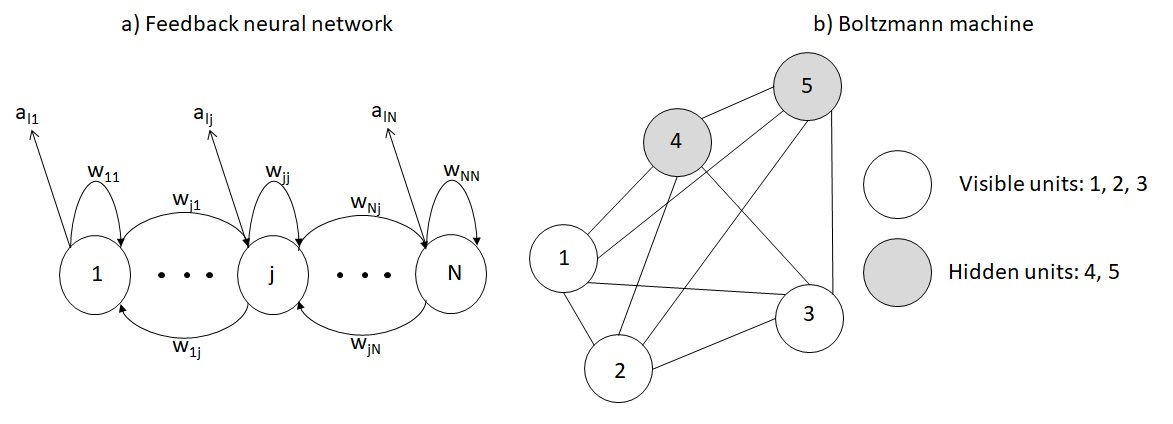
\includegraphics[scale=0.7]{Chapters/Figures/Figure_1_horizontal.jpg}
    \caption{Network architectures a) Feedback neural network b) Boltzmann machine}
    \label{fig:FBNN_n_BM}
\end{figure}

\begin{figure}[h]
    \centering
    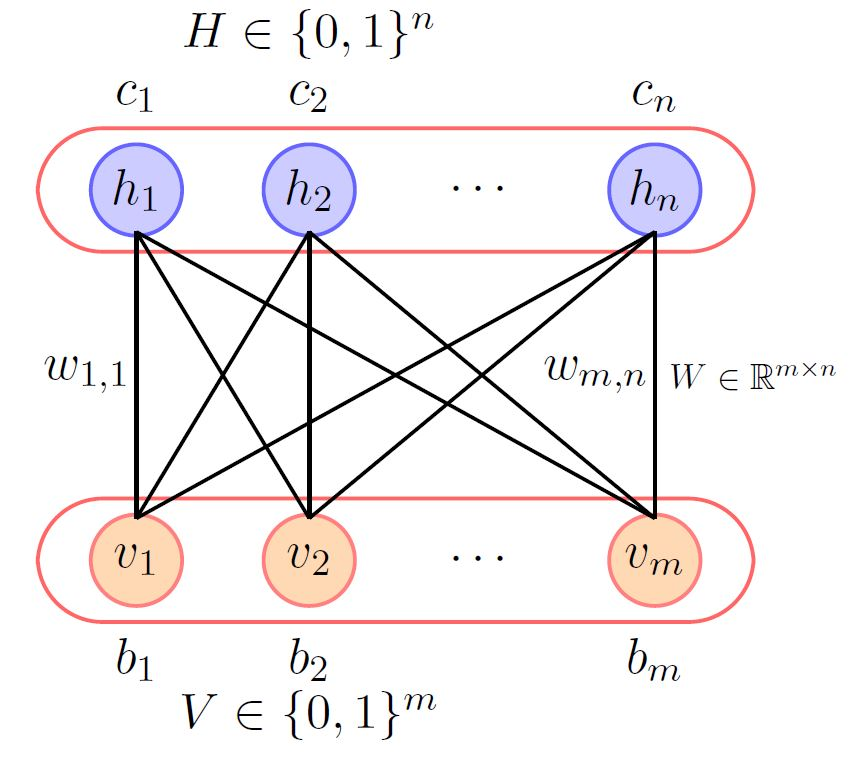
\includegraphics[scale=0.70]{Chapters/Figures/lect_19_slide_43_RBM.JPG}
    \caption{RBM}
    \label{rbm}
\end{figure}





From the feedback network, we can write the equation of energy corresponding to a given state as:
\begin{equation}
    E(V,H)=-\sum_{i}\sum_{j}w_{ij}v_{i}h_{j}-\sum_{i}b_{i}v_{i}-\sum_{j}c_{j}h_{j}
\end{equation}

and the probability of a visible and hidden unit state can be given as:
\begin{equation}
    P(V,H)=\frac{e^{-E(V,H)}}{\sum_{V}\sum_{H}e^{-E(V,H)}}
\end{equation}
where  $V \in \{0,1\}^{m}$, $H \in \{0,1\}^{n}$  for a binary RBM or $V \in R^{m}$, $H \in R^{n}$ for a continuous RBM , m and n is the number of visible and number of hidden units respectively. 
\section{RBM Training}
The training in RBM is unsupervised. Given the data points X as input to the visible units, we have to learn $P(V,H)$ which is parameterized as $ P(V,H)=\frac{e^{-E(V,H)}}{\sum_{V}\sum_{H}e^{-E(V,H)}}$, where the hidden units are unknown. 

As we want to store the pattern $X \in V$ in the network, we have to capture $P(X)$, which can be written as $\sum_{H}P(V,H)$.

So, for a given dataset D ($D=\{x_{1}, x_{2}, ..., x_{l}\}$), we have to maximize $\prod_{i=1}^{l}P(x_{i}|\theta)$, where $\theta$ are the parameters ($w_{ij},c_{i},b_{j}$) of the neural network. 

The objective function can be written as
\begin{equation}
 \begin{aligned}
 ln L(\theta)=&ln \prod_{i=1}^{l}P(x_{i}|\theta)\\
            =&\sum_{i=1}^{l}ln P(x_{i}|\theta)\\
            =&\sum_{i=1}^{l} ln P(V_{i}|\theta)\\
            =&\sum_{i=1}^{l} ln \sum_{H}\frac{e^{-E(V,H)}}{\sum_{V}\sum_{H}e^{-E(V,H)}}
 \end{aligned}
\end{equation}

we have to maximize $ln (L(\theta))$ i.e
$\max_{\theta}\sum_{i=1}^{l} ln \sum_{H}\frac{e^{-E(V,H)}}{\sum_{V}\sum_{H}e^{-E(V,H)}} $. 

We can use stochastic gradient approach to update the parameters of the network, which will maximize the objective function, for that we have to compute $\frac{\partial ln L(\theta)}{\partial \theta}$.
\begin{equation}
    \begin{aligned}
    \frac{\partial ln L(\theta)}{\partial \theta}=&\frac{\partial }{\partial \theta}
    \big[ln \sum_{H}e^{-E(V,H)}-ln \sum_{V,H}e^{-E(V,H)}\big]\\
    =&-\sum_{H}\frac{e^{-E(V,H)}}{\sum_{H}e^{-E(V,H)}}\frac{\partial E(V,H)}{\partial \theta}+\sum_{V,H}\frac{e^{-E(V,H)}}{\sum_{V,H}e^{-E(V,H)}}\frac{\partial E(V,H)}{\partial \theta}\\
    =&-\sum_{H}P(H|V)\frac{\partial E(V,H)}{\partial \theta}+\sum_{V,H}P(V,H)\frac{\partial E(V,H)}{\partial \theta}
    \end{aligned}
\end{equation}

Now our $\theta =\{w_{ij},c_{i},b_{j}\}$, so we have to compute $\frac{\partial ln L(\theta)}{\partial w_{ij}}$, $\frac{\partial ln L(\theta)}{\partial b_{j}}$ and $\frac{\partial ln L(\theta)}{\partial c_{i}}$ one by one.

\begin{equation}
\label{pw}
    \begin{aligned}
    \frac{\partial ln L(\theta)}{\partial w_{ij}}=&\sum_{H}P(H|V)h_{i}v_{j}-\sum_{V,H}P(V,H)h_{i}v_{j}\\
        =&\sum_{H}P(H|V)h_{i}v_{j}-\sum_{V}P(V)\sum_{H}P(H|V)h_{i}v_{j}
    \end{aligned}
\end{equation}
From eq.~\ref{pw} it has been seen that there is common term $\sum_{H}P(H|V)h_{i}v_{j}$ need to be solved.

\begin{equation}
    \begin{aligned}
    \sum_{H}P(H|V)h_{i}v_{j}=&\sum_{H_{i}}P(H_{i}|V)P(H_{-i}|V)h_{i}v_{j}\\                =&\sum_{H_{i}}P(H_{i}|V)h_{i}v_{j}\sum_{H_{-i}}P(H_{-i}|V)\\
                =&P(H_{i}=1|V)v_{j}\\
%               =&\sigma(\sum_{j=1}^{m}w_{ij}+c_{i})v_{j}
    \end{aligned}
\end{equation}

The $P(H_{i}=1|V)$ can be written as:
\begin{equation}
    \begin{aligned}
    P(H_{i}=1|V)=&P(H_{i}=1|H_{-i},V)\\
                =&\frac{e^{-E(H_{i}=1,H_{-i},V)}}{e^{-E(H_{i}=1,H_{-i},V)}+e^{-E(H_{i}=0,H_{-i},V)}}\\
                =&\frac{1}{1+e^{-(-\sum_{l}w_{li}v_{l}-c_{i})}}\\
                =&\sigma({\sum_{l}w_{li}v_{l}+c_{i}})
    \end{aligned}
\end{equation}
Now, $\frac{\partial ln L(\theta)}{\partial w_{ij}}$ can be written as:
\begin{equation}
    \begin{aligned}
    \frac{\partial ln L(\theta)}{\partial w_{ij}}=&\sigma({\sum_{j}w_{ij}v_{j}+c_{i}})v_{j}-\sum_{V}P(V)\sigma({\sum_{j}w_{ij}v_{j}+c_{i}})v_{j}\\
    \nabla_{w}L(\theta)=&\sigma(WV+C)V^{T}-\sum_{V}P(V)\sigma(WV+C)V^{T}\\
    \nabla_{w}L(\theta)=&\sigma(WV+C)V^{T}-E_{V}[\sigma(WV+C)V^{T}]
    \end{aligned}
\end{equation}

Similarly, $\nabla_{b}L(\theta)$, $\nabla_{c}L(\theta)$ can be written as,
\begin{equation}
    \begin{aligned}
    \nabla_{b}L(\theta)=&V-E_{v}[v]\\
    \nabla_{c}L(\theta)=&\sigma(WV+C)-E_{V}[\sigma(WV+C)]
    \end{aligned}
\end{equation}
From the equations of $\nabla_{w}L(\theta)$, $\nabla_{b}L(\theta)$ and $\nabla_{c}L(\theta)$, there are three expectation terms in all the cases, which require us to compute the expectation over all the possible states of all visible units. If we consider V to take only binary values; the possible number of state sequence will be $2^{m}$ which increases exponentially with increase in the number of visible unit $m$. In general, to compute the expectation instead of using all population (possible states) sample of states can be used. The samples are drawn using \textbf{Gibbs Sampling} (uses Markov chain property to learn the stationary distribution). Suppose $k$ is number of steps require to get the stationary distribution, then generate $r$ number of samples from the stationary distribution and take the average of that to compute the expectation terms. Hence the expectation terms can be rewritten as:

\begin{equation}
    \begin{aligned}
    E_{V}[\sigma(WV+C)V^{T}]=&\frac{1}{r}\sum_{i=k+1}^{k+r}\sigma(WV^{(i)}+C)V^{(i)T}\\
    E_{V}[V]=&\frac{1}{r}\sum_{i=k+1}^{k+r}V^{(i)}\\
    E_{V}[\sigma(WV+C)]=&\frac{1}{r}\sum_{i=k+1}^{k+r}\sigma(WV^{(i)}+C)
    \end{aligned}
\end{equation}

Finally the update equation can be written as using Gibbs sampling as:
\begin{equation}
    \begin{aligned}
    W=&W+\sigma(WV_{d}+C)V_{d}^{T}-\frac{1}{r}\sum_{i=k+1}^{k+r}\sigma(WV^{(i)}+C)V^{(i)T}\\
    b=&b+V_{d}-\frac{1}{r}\sum_{i=k+1}^{k+r}V^{(i)}\\
    C=&C+\sigma(WV_{d}+C)-\frac{1}{r}\sum_{i=k+1}^{k+r}\sigma(WV^{(i)}+C)
    \end{aligned}
\end{equation}
where W,b,C, $V_{d}$ and V are the weight, bias visible unit, bias hidden unit, training input data (to visible unit) sampled state (corresponding to visible unit) respectively. The full algorithm of RBM training using Gibbs sampling is depicted in Fig.~\ref{fig:rbm_algo}.



\begin{figure}[h]
    \centering
    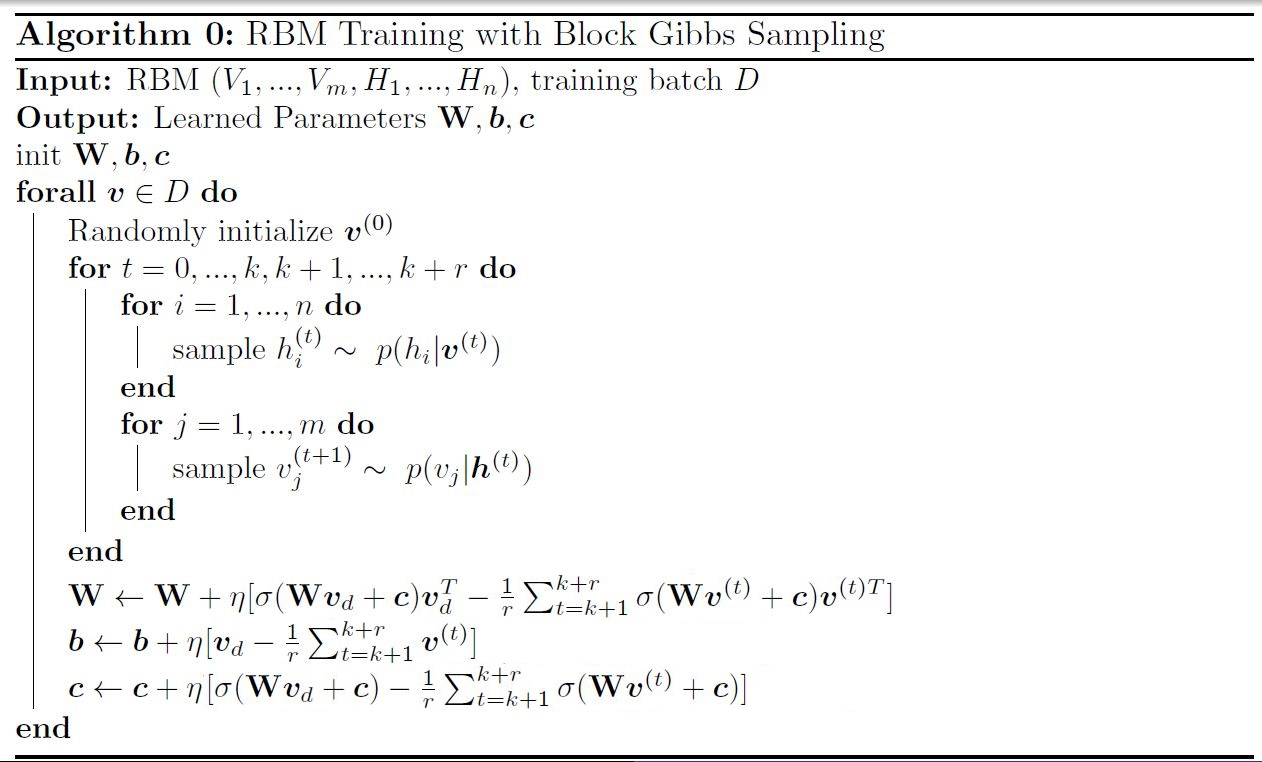
\includegraphics[scale=0.65]{Chapters/Figures/lect_20_slide_54_RBM_algorithm.JPG}
    \caption{RBM Algorithm}
    \label{fig:rbm_algo}
\end{figure}

The drawback of the Gibbs sampling based approach is that, it could take many iterations $(k)$ to reach the stationary distribution since we initialize $V^{0}$ randomly. There is an approach called k-contrastive divergence approach, where the $V^{0}$ is initialized to the current training data sample $V_{d}$ following which, the vanilla Gibbs Sampling is run. for k steps. Let the sample at the $k^{th}$ step be denoted by $\tilde{V}$(refer Fig.~\ref{fig:Conrastive_divergence}). 

\begin{figure}[h]
    \centering
    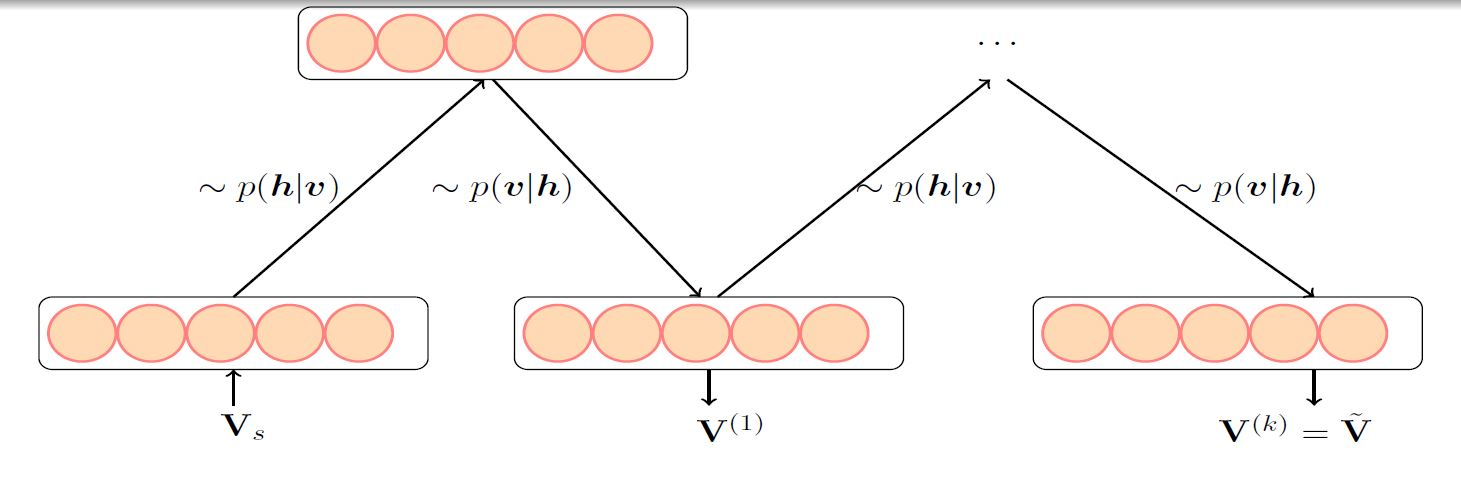
\includegraphics[scale=0.6]{Chapters/Figures/lect_20_slide_58_Conrastive_divergence.JPG}
    \caption{Contrastive divergence}
    \label{fig:Conrastive_divergence}
\end{figure}

The update rule for k-contrastive divergence approach can be written as per eq.~\ref{kcd}:
\begin{equation}
\label{kcd}
    \begin{aligned}
    W=&W+\sigma(WV_{d}+C)V_{d}^{T}-\sigma(W\tilde{V}+C)\tilde{V^{T}}\\
    b=&b+V_{d}-\tilde{V}\\
    C=&C+\sigma(WV_{d}+C)-\sigma(W\tilde{V}+C)
    \end{aligned}
\end{equation}

In practice $k=1$ is work fine. The detailed algorithm to train RBM using  k-contrastive divergence approach is depicted in Fig.~\ref{fig:Conrastive_divergence_algo}.




\begin{figure}[h]
    \centering
    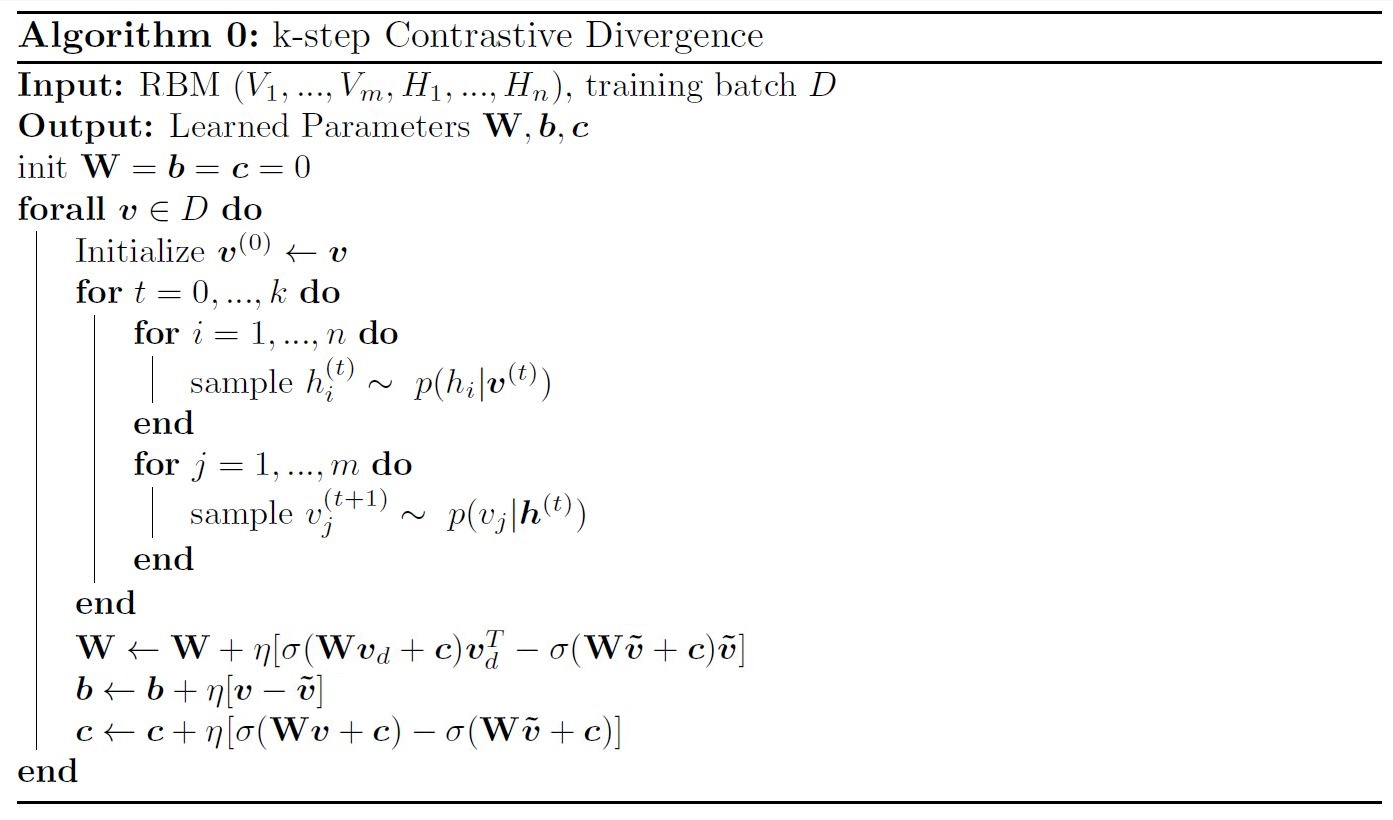
\includegraphics[scale=0.65]{Chapters/Figures/lect_20_slide_60_Conrastive_divergence_algo.JPG}
    \caption{Conrastive divergence algorithm}
    \label{fig:Conrastive_divergence_algo}
\end{figure}










\end{spacing} 